\subsection{bestLDS provides good initializations for EM}
\label{sec:bestlds:results:4.2}

In regimes where additional accuracy is desired, bestLDS may serve as smart initializations for EM. Indeed, estimates returned by spectral estimators have previously been shown to serve as good EM initialization points \cite{martens_learning_2010, buesing_spectral_2012}. This is particularly important given that EM fitting procedures typically require the user to initialize randomly (or at least, without complete knowledge of what a good initialization would be) and therefore a single fit is rarely sufficient to determine that EM has found the global optimum. Instead, users often fit EM to their data many times and take the parameters from those that produced the highest log-likelihood or ELBO (Evidence Lower Bound). This can be extremely time-consuming, especially when datasets are large. Thus, a method that can generate initializations that (1) converge quickly and (2) consistently converge to the global optimum can substantially reduce compute-time.

\begin{figure*}[t!]
\centering
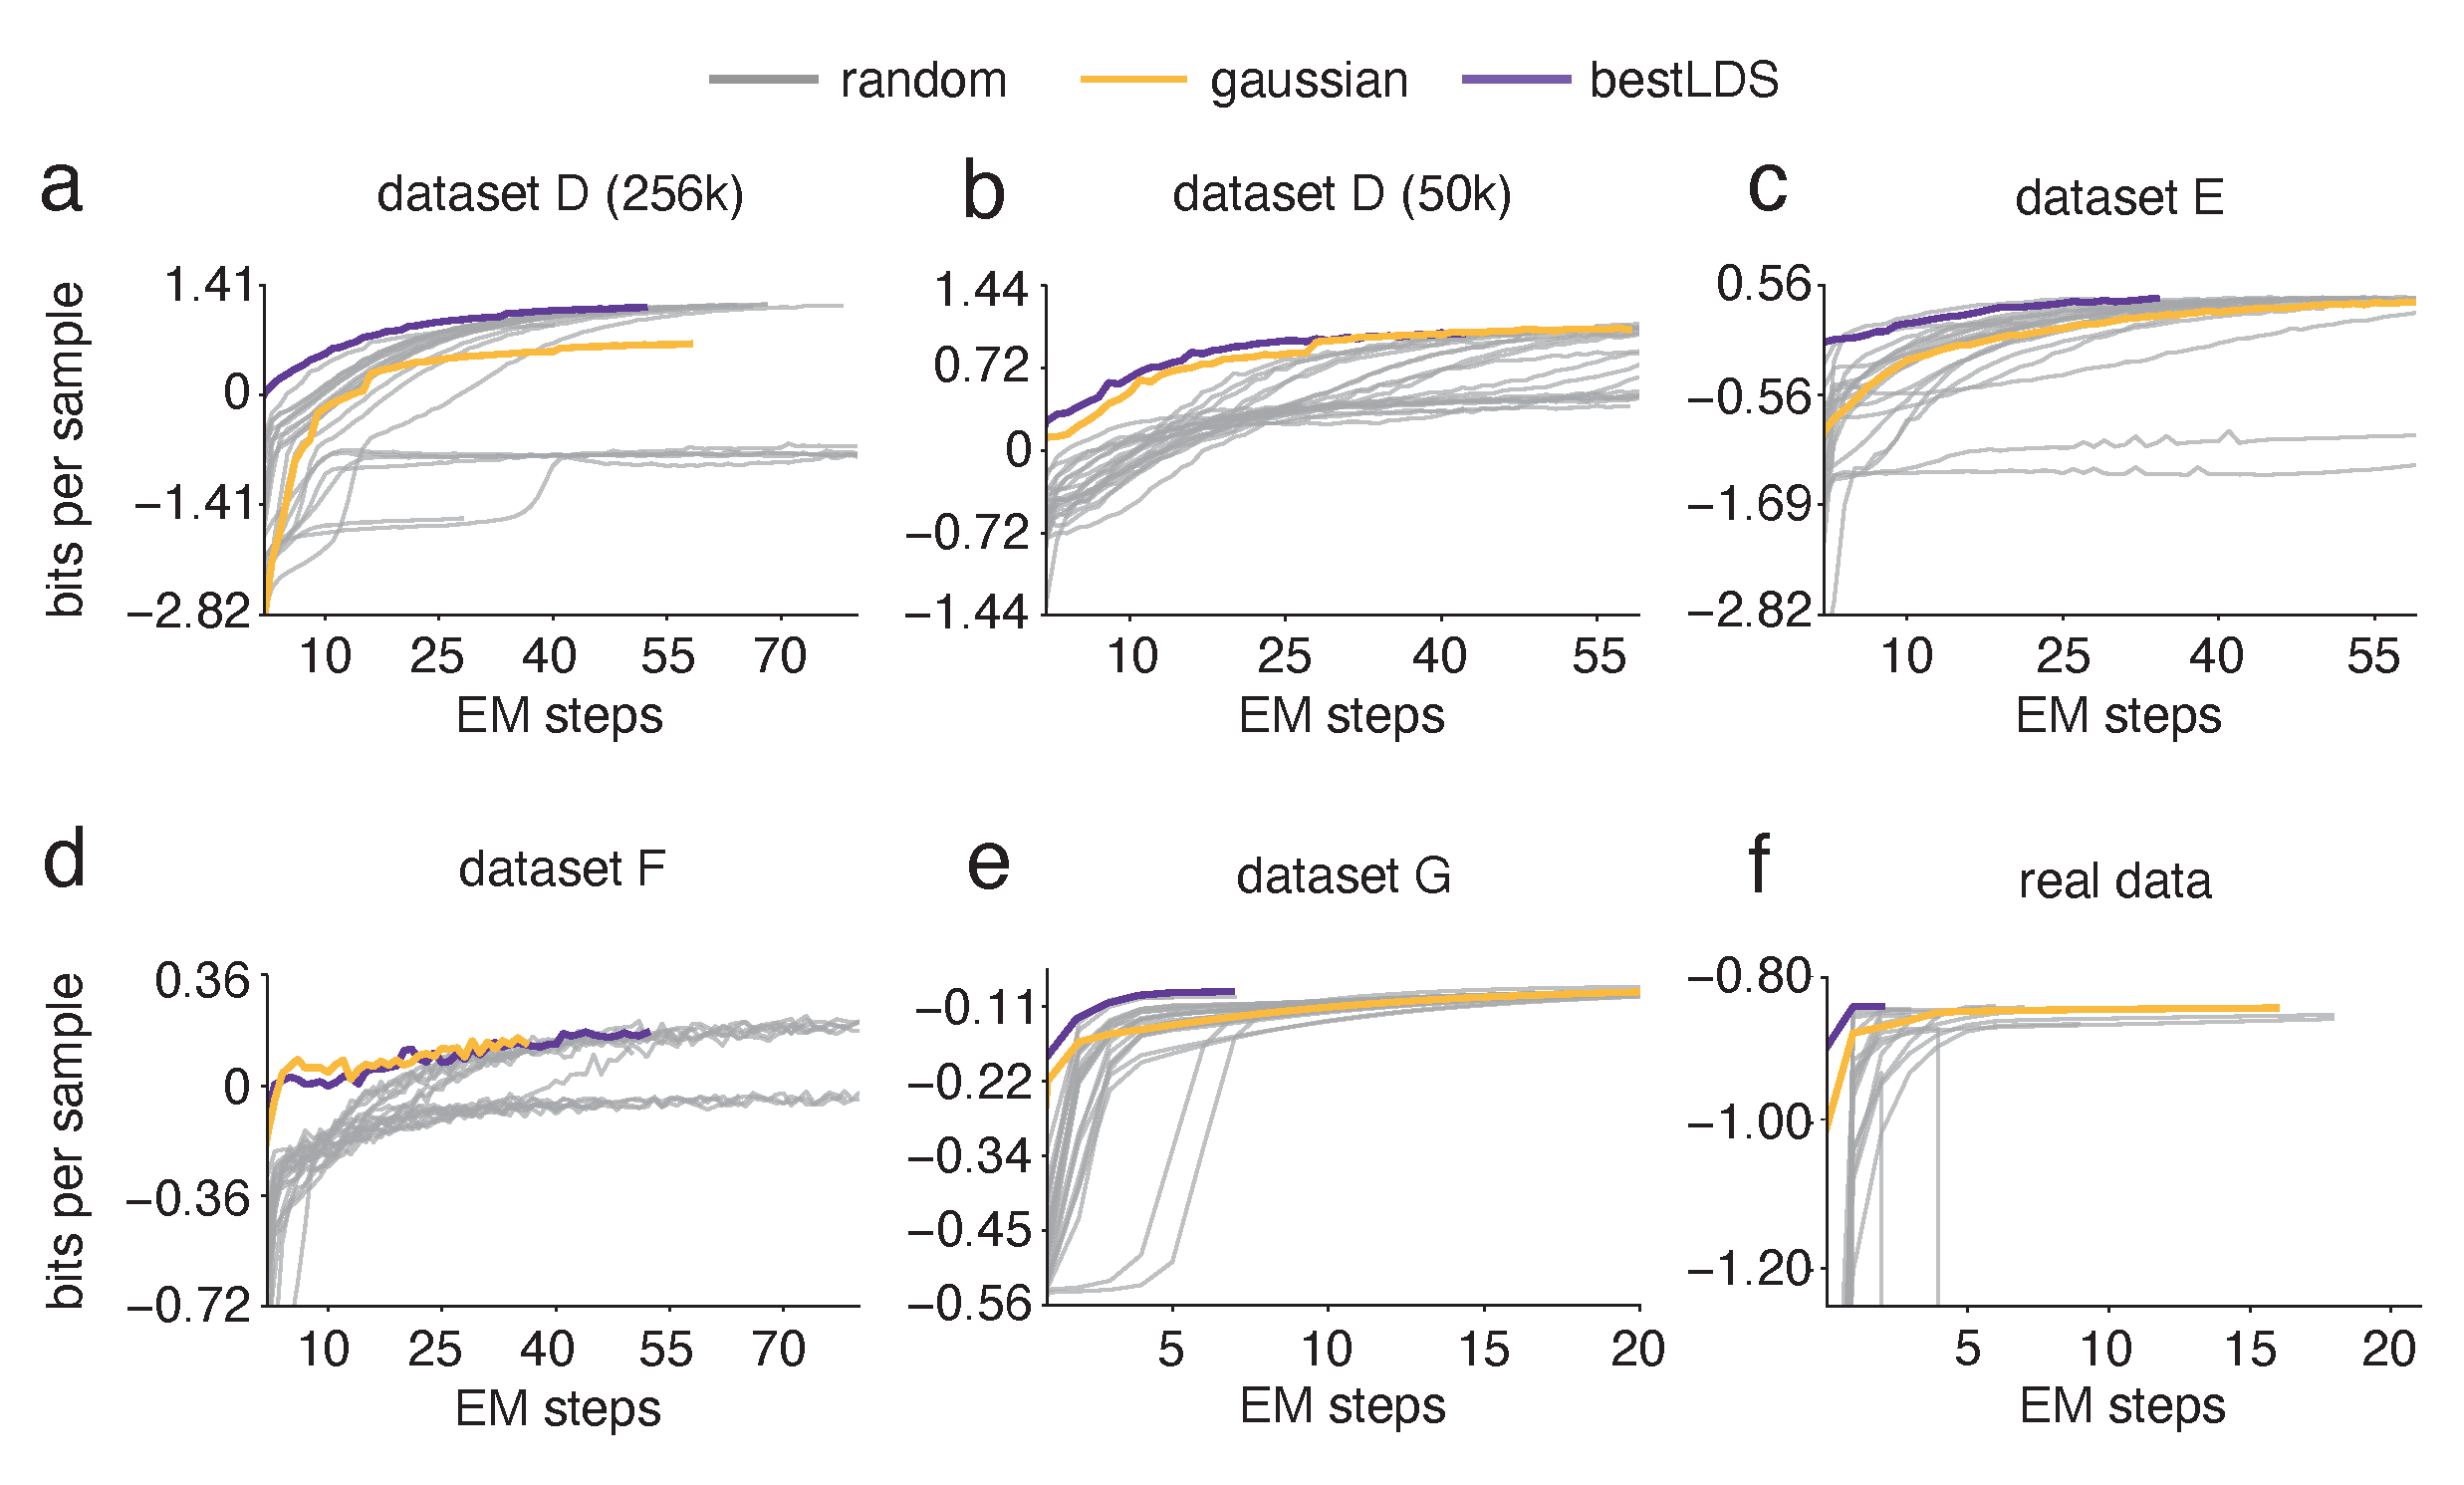
\includegraphics[width=0.90\linewidth]{ch4-bestlds/bestlds-figures/fig3.pdf}
%\vspace{-0.3cm}
\caption{\textbf{bestLDS is an effective initialization for EM.} For panels a-d, the ELBO (converted to bits/sample) is plotted on each step of EM with random initializations, a bestLDS initialization, and a Gaussian initialization. Panels e-f are the same except that EM returns the log-evidence at each step. \textbf{(a)} Dataset D is characterized by slow rotational dynamics and high-magnitude output matrix. It exhibits long stretches of 0s and 1s. Inputs were drawn from a zero-mean normal distribution with covariance $\Sigma_u = 10^{-4}I$. \textbf{(b)} Same as (a) but with $N=50,000$. \textbf{(c)} Dataset E is characterized by extremely fast rotational dynamics. It exhibits switching behavior, alternating emissions of 0s and 1s. Inputs were drawn from a zero-mean normal distribution with covariance $\Sigma_u = 0.1I$. \textbf{(d)} Dataset F is similar to dataset B but has inputs sampled from a Student-t distribution with three degrees of freedom. \textbf{(e)} Dataset G has one-dimensional observations ($q=1$) with slow rotational dynamics. See Appendix Table \ref{table:ap2:1} for more details on all simulation parameters. \textbf{(f)} Data taken from mice performing a two-alternative forced choice task in virtual reality. See Section~\ref{sec:bestlds:results:4.3} for details. }
\label{fig:bestlds:3}
%\vspace{-0.4cm}
\end{figure*}

Accordingly, we examined how useful bestLDS is in such a role. In this section we assess the performance of this estimator as an initialization for Laplace-EM\footnote{Implemented using the Python ssm package, licensed under the MIT license}, an EM method using the Laplace approximation to efficiently compute the log posterior \cite{smith_estimating_2003, kulkarni_common-input_2007, paninski_new_2010, yuan_estimating_2010}. We then compare the results to random and linear-Gaussian\footnote{using the same process as described in the model comparisons section} initializations when fit to three different simulated datasets. For each dataset and initialization method, we have plotted the ELBO as a function of the number of EM steps taken until the system reaches convergence\footnote{for the $q\geq p$ regime, we say that EM has converged when the avg. $|\Delta|$ in the gain matrix on successive steps is within a tolerance ($tol=0.15$); for $p<q$ we found that comparing the log-evidence on successive steps to be more reliable ($tol=10$, in bits/sample).}---this is a useful metric to examine since our primary interest is training time and not performance. For the sake of clarity, we will briefly describe each dataset considered for this purpose and have provided a full accounting of all the generative parameters in Appendix Table \ref{table:ap2:1}.

First, we examined the case in which the dimensionality of the outputs was greater than that of the latents (i.e., $q > p$). In particular, we considered datasets exhibiting properties that one might expect from typical Bernoulli datasets (e.g., mouse decision-making behavior). For example, dataset D is characterized by long stretches of $0$s or $1$s, which we might expect in behavioral datasets that exhibit high autocorrelation (e.g., habitual behaviors, perseveration, etc.); this was implemented by imposing slow rotational dynamics. Here, the bestLDS initialization substantially outperforms Gaussian and random initializations, eliciting higher ELBOs from the first step of EM and converging to the optimal solution in fewer total steps (Figure~\ref{fig:bestlds:3}a), thus saving notable computation time (Table~\ref{table:bestlds:2}, top, first column). This result also holds for the same dataset fit to fewer data points (Figure~\ref{fig:bestlds:3}b). In this case, while the Gaussian initialization also achieves the global optimum, it still takes more time to converge than the bestLDS initialization and in fact offers negligible time-savings over the average random initialization (Table~\ref{table:bestlds:2}, top, second column). Dataset E reflects a different extreme of Bernoulli-distributed behavior in that it produces observations that rapidly switch between $0$s and $1$s, which we implement by imposing fast rotational dynamics. We might expect this type of data from alternation tasks (i.e., the subject must make the opposite choice from the previous trial). The bestLDS initialization significantly aids performance on this dataset as well (Figure~\ref{fig:bestlds:3}c) and reduces convergence time over Gaussian initializations by approximately 50$\%$ (Table~\ref{table:bestlds:2}, top, third column). Finally, dataset F is almost identical to dataset B (see Figure~\ref{fig:bestlds:2} and Table~\ref{table:bestlds:1}) except that inputs are drawn from a Student-t distribution with three degrees of freedom, thus testing the flexibility of our assumptions on the input sampling distribution. Here we find that both non-random initializations perform well, indicating the general utility of these spectral methods on input-output data even when the inputs are non-Gaussian (Figure~\ref{fig:bestlds:3}d and Table~\ref{table:bestlds:2}, bottom, first column).

\begin{table*}[t!]
\setlength{\tabcolsep}{5pt}
\centering
\caption[Time to convergence for Laplace-EM for different initialization methods]{\textbf{Time to convergence for Laplace-EM for different initialization methods.} For random initializations ($N=20$), both total and mean (total / mean) times are reported. For bestLDS initializations, we report both the time to convergence and the time to acquire the initializations using the bestLDS estimator (estimator time + convergence time). All computations were performed on an internal CPU cluster.}
\vspace{0.2cm}
 \begin{tabular}{|p{2.7cm}||p{3.5cm}|p{3.5cm}|p{3.5cm}|}
 \hline
 \multicolumn{4}{|c|}{\textbf{Convergence Times for Laplace-EM} (min.) } \\
 \hline
 \textbf{Initialization} & \textbf{Dataset D} ($256$k) & \textbf{Dataset D} ($50$k) & \textbf{Dataset E} ($256$k) \\ 
 \hline
 \textbf{random} &   902 / 45.10  & 232.40 / 11.62   & 571.75 / 28.09  \\
 \textbf{Gaussian} &   38.67  & 11.60  & 39.67 \\
 \textbf{bestLDS}    & 0.15 + 34.67 & 0.09 + 8.40 &  0.14 + 19.83  \\
 \hline
 \textbf{Initialization} & \textbf{Dataset F} ($100$k) & \textbf{Dataset G} ($256$k) & \textbf{Real Data} ($54883$) \\ 
 \hline
 \textbf{random} &   514.33 / 25.72  & 886.67 / 44.33   & 25.11 / 1.67 \\
 \textbf{Gaussian} &   12.67  & 49.40  & 5.61  \\
 \textbf{bestLDS}    & 0.10 + 19.67 & 0.05 + 8.87 &  0.02 + 0.33  \\
 \hline
\end{tabular}
\label{table:bestlds:2}
%\vspace{-0.3cm}
\end{table*}

Next, we turned our attention to the $q < p$ case, specifically focusing on when $q = 1$ due to its practical relevance for neuroscience decision-making experiments, in which subjects are more likely to undergo tasks one-by-one and elicit a single choice output at a time. Dataset G is a simulated dataset in this regime, characterized by slow rotational dynamics. As earlier, the bestLDS estimate attains a higher log-evidence than comparative methods from the first step of EM (Figure~\ref{fig:bestlds:3}e) and converges much faster than the Gaussian or random initializations (roughly a factor of 5.5 faster; see Table~\ref{table:bestlds:2}, bottom, second column). Finally, we performed these comparisons on binary data from mice performing a decision-making task (see Section \ref{sec:bestlds:results:4.3}). Here, the bestLDS initialization converges in only three steps of EM (Figure~\ref{fig:bestlds:3}f). All other initializations take significantly longer to converge (on the order of 17x slower for Gaussian LDS, and 76x slower for the random initialization total time; see Table~\ref{table:bestlds:2}, bottom, third column), and also have initial log-evidence values that are noticeably lower than the bestLDS estimate.